\section{L and NL}

Sublinear space bounds where $f(n)$ is much smaller than $n$. This won't make sense given our existing one-tape Turing machine model since we won't even have enough space to store the input.

We modify our model and have a 2-tape Turing machine where we have one tape as a read-only input tape, and another tape as the read/write work tape. We don't have to store all data on the main memory, so we would like to consider \textit{only the computation spaced used on the work tape}.

$$
\LSpace = \Space(\log n)
$$
$$
\NLSpace = \NSpace(\log n)
$$

Savitch's theorem still holds, so $\NLSpace \subseteq \Space(\log^2 n)$.

\begin{theorem}
    $
    \LSpace \subseteq \p
    $
\end{theorem}

\begin{proof}
    Let $A$ be a language in $\LSpace$. There exsits some logspace-bounded 2-tape TM $M$ that decides $A$. We define the configuration for a logspace-bounded 2-tape Turing machine $M$ on $w$ as $(q,p_1,p_2,t)$ where $q$ is a state, $p_1$ and $p_2$ are the tape positions (for the read-only input tape and work tape, respectively), and $t$ is the tape content on the work tape. Then, the number of possible configurations is $|Q| \times n \times O(\log n) \times |\Gamma|^{O(\log n)} = O(n^k)$ for some $k$. Therefore, $M$ runs in polynomial time.
\end{proof}

\section{PATH is in NL}

$$
\text{PATH} = \{ \encoding{G,s,t} \mid \text{$G$ has directed path from $s$ to $t$ } \}
$$

\begin{theorem}[PATH in NL]
    $$
    \text{PATH} \in \NLSpace
    $$
\end{theorem}

\begin{proof}
    At each vertex, we use nondeterminism to guess the next vertex. Suppose we have the path $p = s s_1 s_2 \ldots t$. At each vertex $s_i$, we look at the next vertex $s_{i+1}$ and checks if $s_{i+1}$ is connected to $s_i$. If any of the nondeterministic paths lead to $t$. At any time during the computation of one nondeterministic path, we have at most the name of two vertices on the work tape. In addition, we keep track of the vertices visited, using $\log n$ space since any simple path contains at most $n$ vertices. It takes at most $\log n$ space to write down the name of a vertex, so PATH $\in \NLSpace$.
\end{proof}

We do not know if PATH $\overset{?}{\in} \LSpace$. We also don't know if $\LSpace \overset{?}{=} \NLSpace$.

\section{NL-Complete}

A language $A$ is in $\NLSpace$-complete if $A \in \NLSpace$ and for all $B \in \NLSpace$, $B \leq_L A$. The symbol $\leq_L$ stands for log-space reducible, which we will define here.

As we will show later, all problems in $\NLSpace$ are also in $\p$. It does not make a lot of sense to define $\NLSpace$-complete in terms of polytime reduction. Note that for all $A,B \in \NLSpace$ except $\emptyset$ and $\Sigma^*$, $A \leq_p B$ and $B \leq_p A$. We need a type of reduction that is more restrictive than polytime reduction.

\subsection{Log-Space Reduction}

A log-space transducer is a Turing machine with
\begin{itemize}
    \item read-only input tape
    \item write-only output tape (head can only move to the right)
    \item read/write work tape (only $O(\log n)$ symbols)
\end{itemize}
that computes a function $f:\; \Sigma^* \to \Sigma^*$ where $f(w)$ is written on output tape when $M$ halts when $w$ is on the input tape.

We say $f$ is a log-space computable function.

\begin{figure}[htbp]
    \centering
    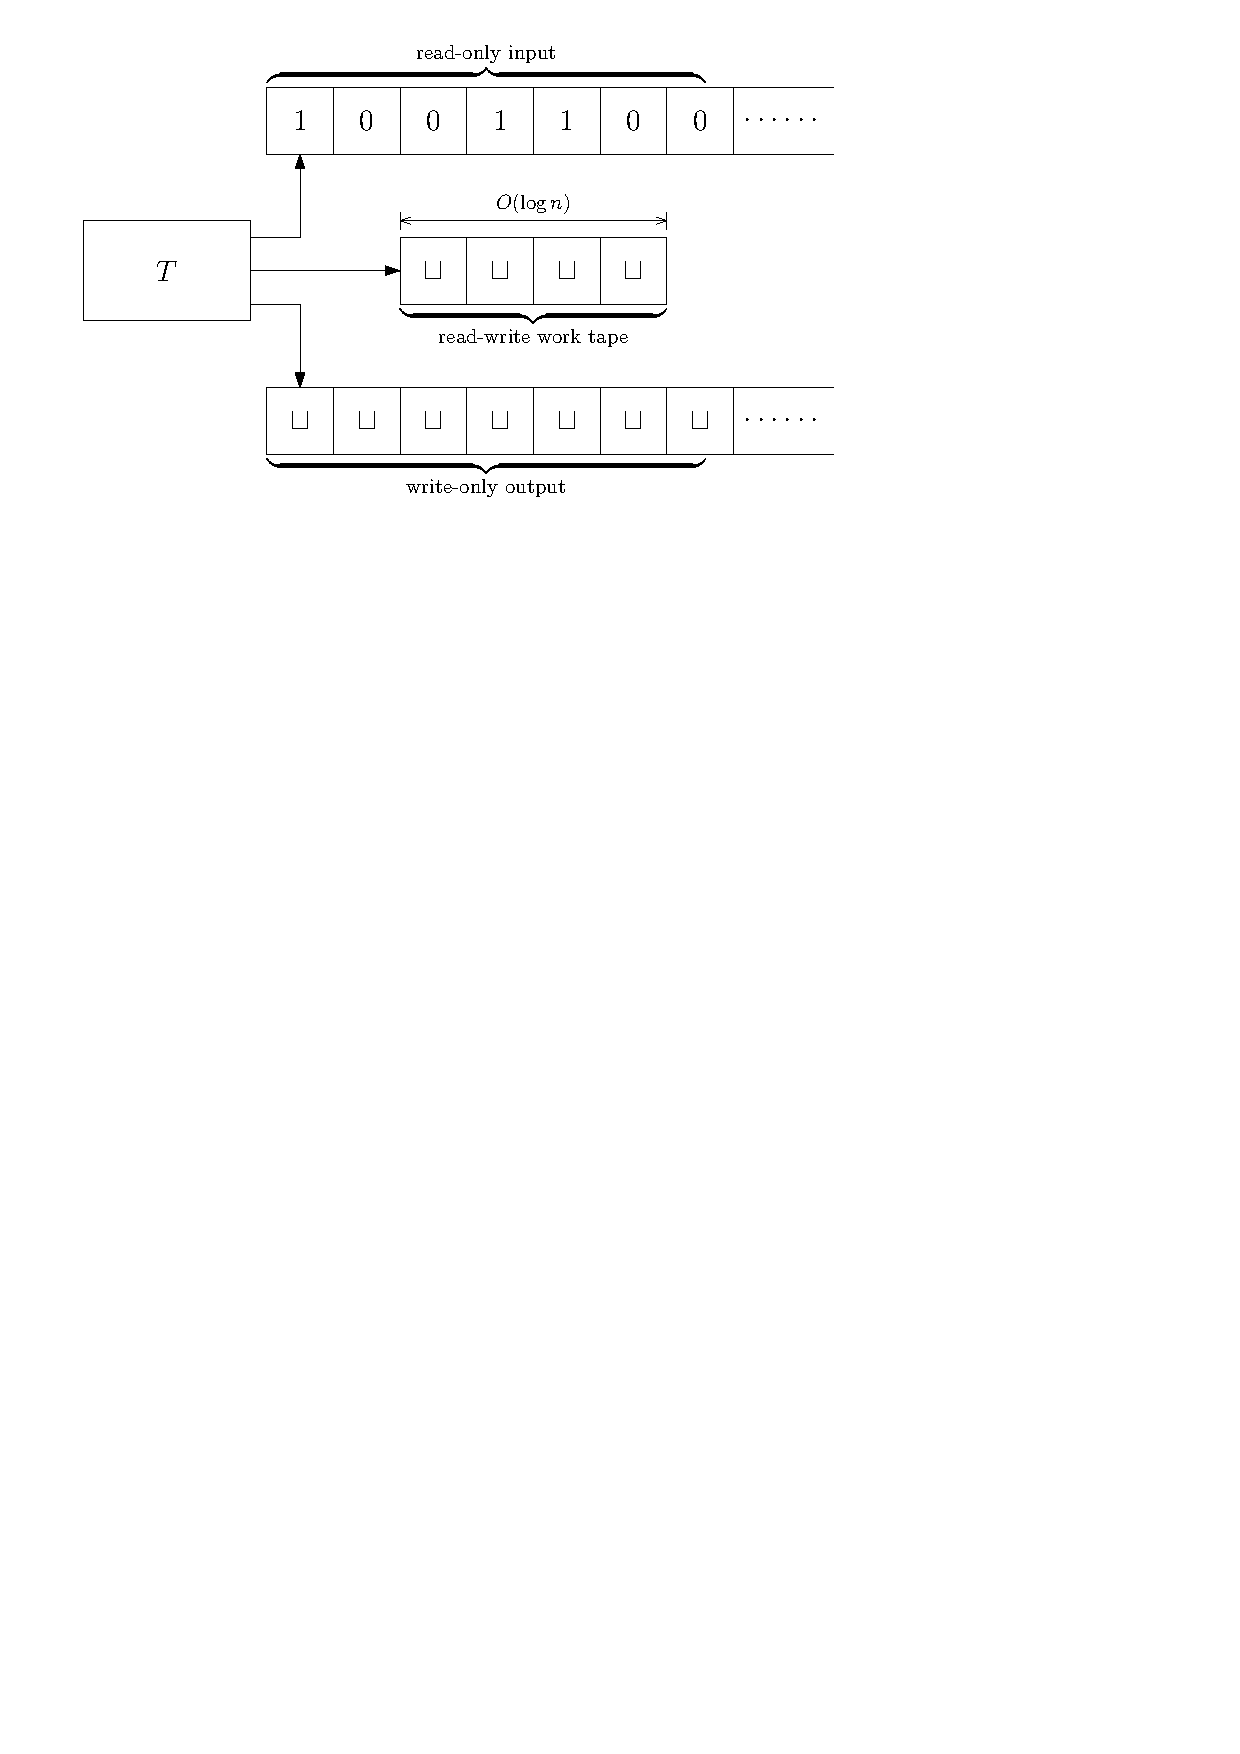
\includegraphics[width=0.4\linewidth]{logspace-transducer.pdf}
    \caption{A log-space transducer}
    \label{fig:logspace-transducer}
\end{figure}

\begin{theorem}
    if $A \leq_L B$ and $B \in \LSpace$, then $A \in \LSpace$.
\end{theorem}

\begin{proof}
    Suppose there exists a log-space decider $M_B$ for $B$. We construct a log-space decider for $A$. A seemingly obvious construction would be:

    \begin{turing}{M}{on input $w$}
        \item run $w$ on the log-space transducer to compute $f(w)$ 
        \item run $M_B$ on $f(w)$ 
    \end{turing}

    The issue with this construction is that we don't have enough space to actually write down the entirety of $f(w)$, so this construction won't quite work.

    We use this algernative construction. Whenever $B$ needs a bit of $f(w)$, we recompute it on the fly. More formally, $M_A$ computes individual symbols of $f(w)$ by calling the logspace transducer as requested by $M_B$. In the simulation, we run $M_B$ without actual input on the tape. When it requests the $i$th bit of the input, we run $M_A$ with a counter to get the $i$th bit of $f(w)$.

    To see why this construction of $M_A$ runs in logspace, observe first that $M_A$ itself needs to keep track of the position requested by $M_B$ when calling the transducer, which takes $O(\log n)$ space. In addition, $M_B$ uses $O(\log |f(w)|) + 1$ space (the one additional bit is used to store the bit requested by $M_B$ at each step of its computation) when we simulate $M_B$. Since $f(w)$ has length of as most the number of configurations that the transducer can have, which is $|w| 2^{O(\log |w|)}$. It follows that the space used by $M_B$ is also in $O(\log |w|) = O(\log n)$. Therefore, $M_A$ runs in logspace.
\end{proof}

\subsection{PATH is NL-Complete}

\vspace{\parskip}

\begin{theorem}
    PATH is $\NLSpace$-complete.
\end{theorem}

\begin{proof}
    We have shown that PATH is in $\NLSpace$. It reamins to be shown that for every language $A \in \NLSpace$, $A \leq_L$ PATH.

    Let $A \in \NLSpace$. There exists a nondeterministic log-space Turing machine $M$ that decides $A$. Given a string $w$, we want to reduce it to a graph representing the computation of $M$ on $w$ where:
    \begin{itemize}
        \item nodes: various configurations
        \item edges: $(c_1,c_2) \in E$ if $c_1$ yields $y_2$  
    \end{itemize}
    Why is this construction log-space computable? We need to give a log-space transducer that outputs $\encoding{G,s,t}$ on input $w$. Note that when constructing a log-space transducer, we don't actually care about the time complexity of the transducer, although the construction that we are about to show is both log-space and runs in polytime. The transducer needs to do two things:

    \begin{enumerate}
        \item List the nodes: This is relatively easy. Each node is a configuration of $M$ on $w$ which can be represented in $c \log n$ space for some constant $c$. The transducer can simply go through every strings of length $c \log n$ using brute force, checks if it encodes a legal configuration of $M$ on $w$, and outputs those that do. This runs in log-space because at any time, we only write at most one string on the work tape.
        \item List the edges: We list the edges of the graph by testing every pair of possible configurations $(c_1,c_2)$ and checks if $c_1$ yields $c_2$. This can be done using log-space as well because we only need to write $c_1$, $c_2$ on the work tape while looking at the transition table to determine if $c_1$ yields $c_2$.
    \end{enumerate}

    \begin{figure}[htbp]
        \centering
        \subfloat{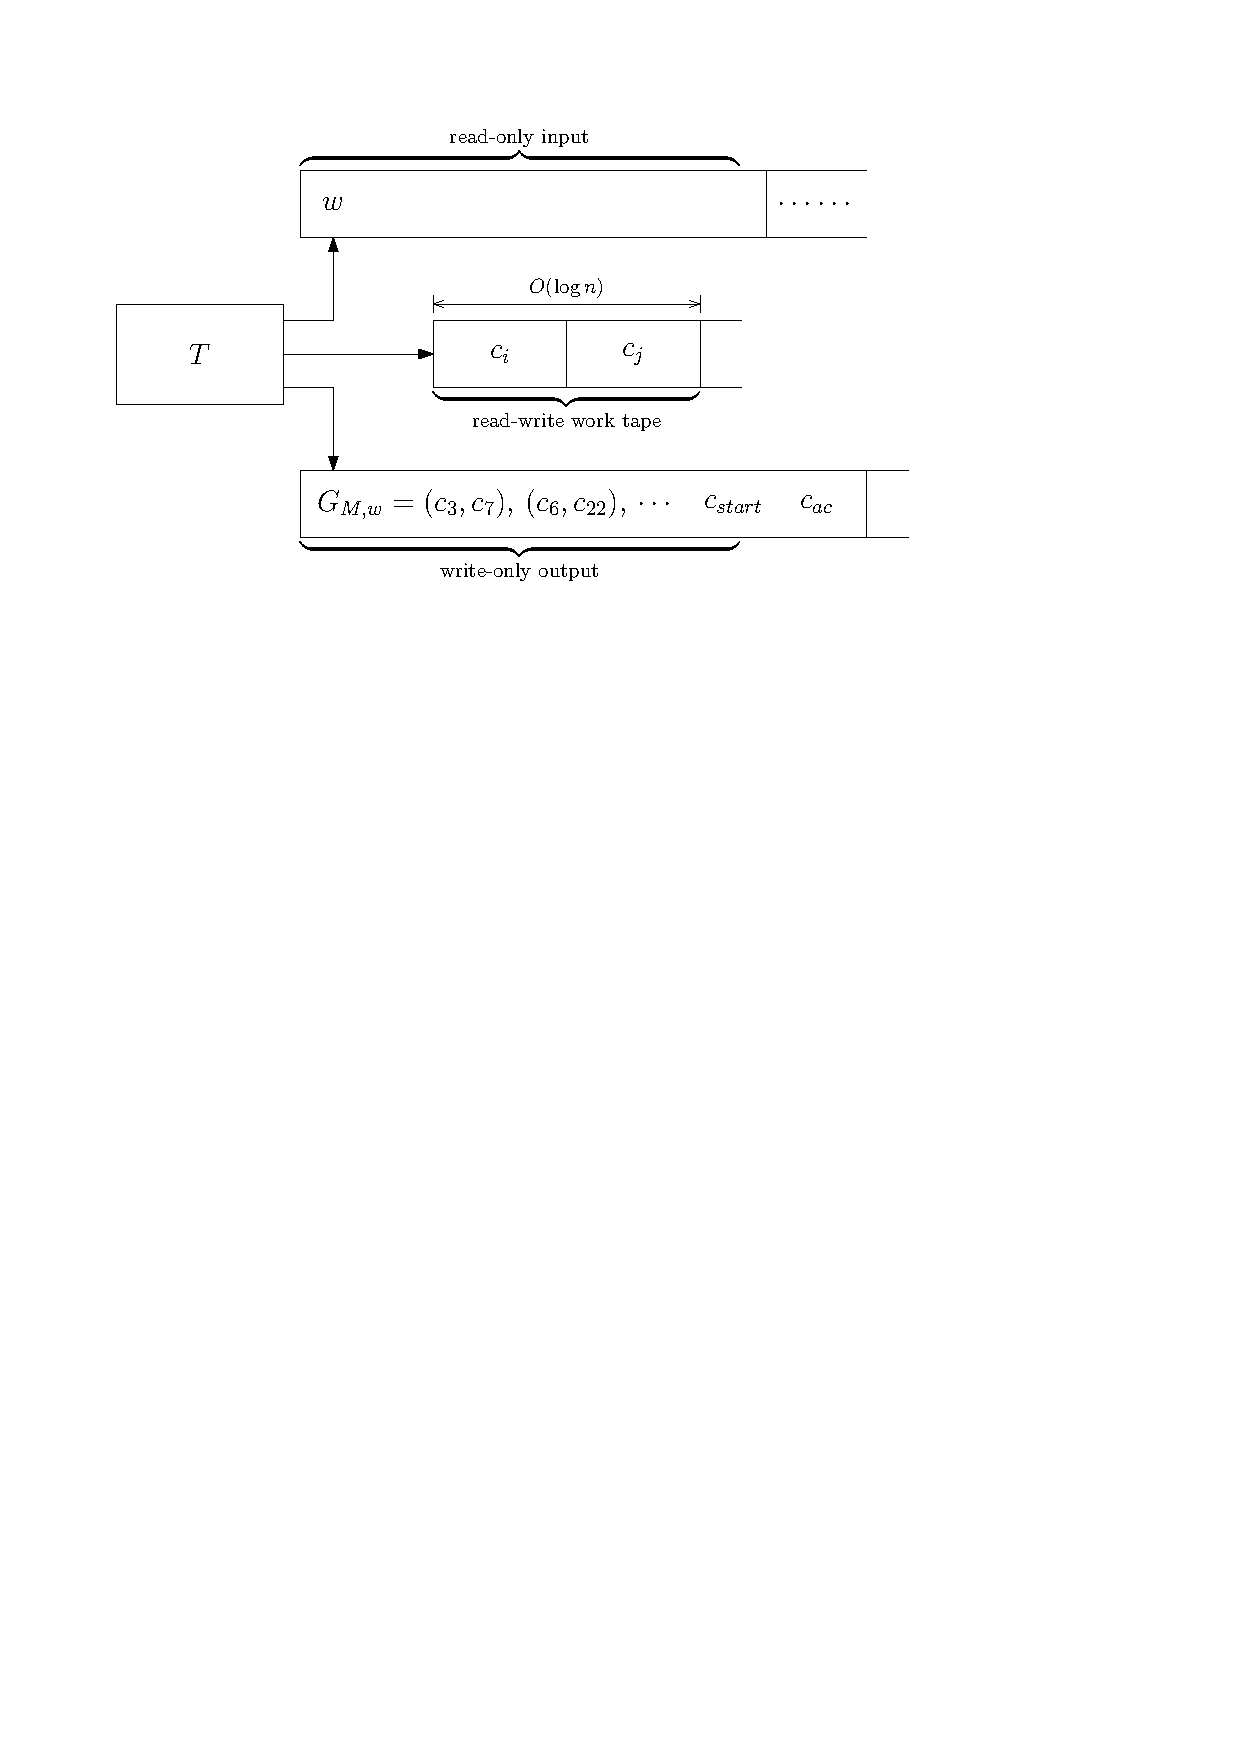
\includegraphics[width=0.5\linewidth,align=c]{logspace-transducer-path.pdf}}
        \qquad
        \subfloat{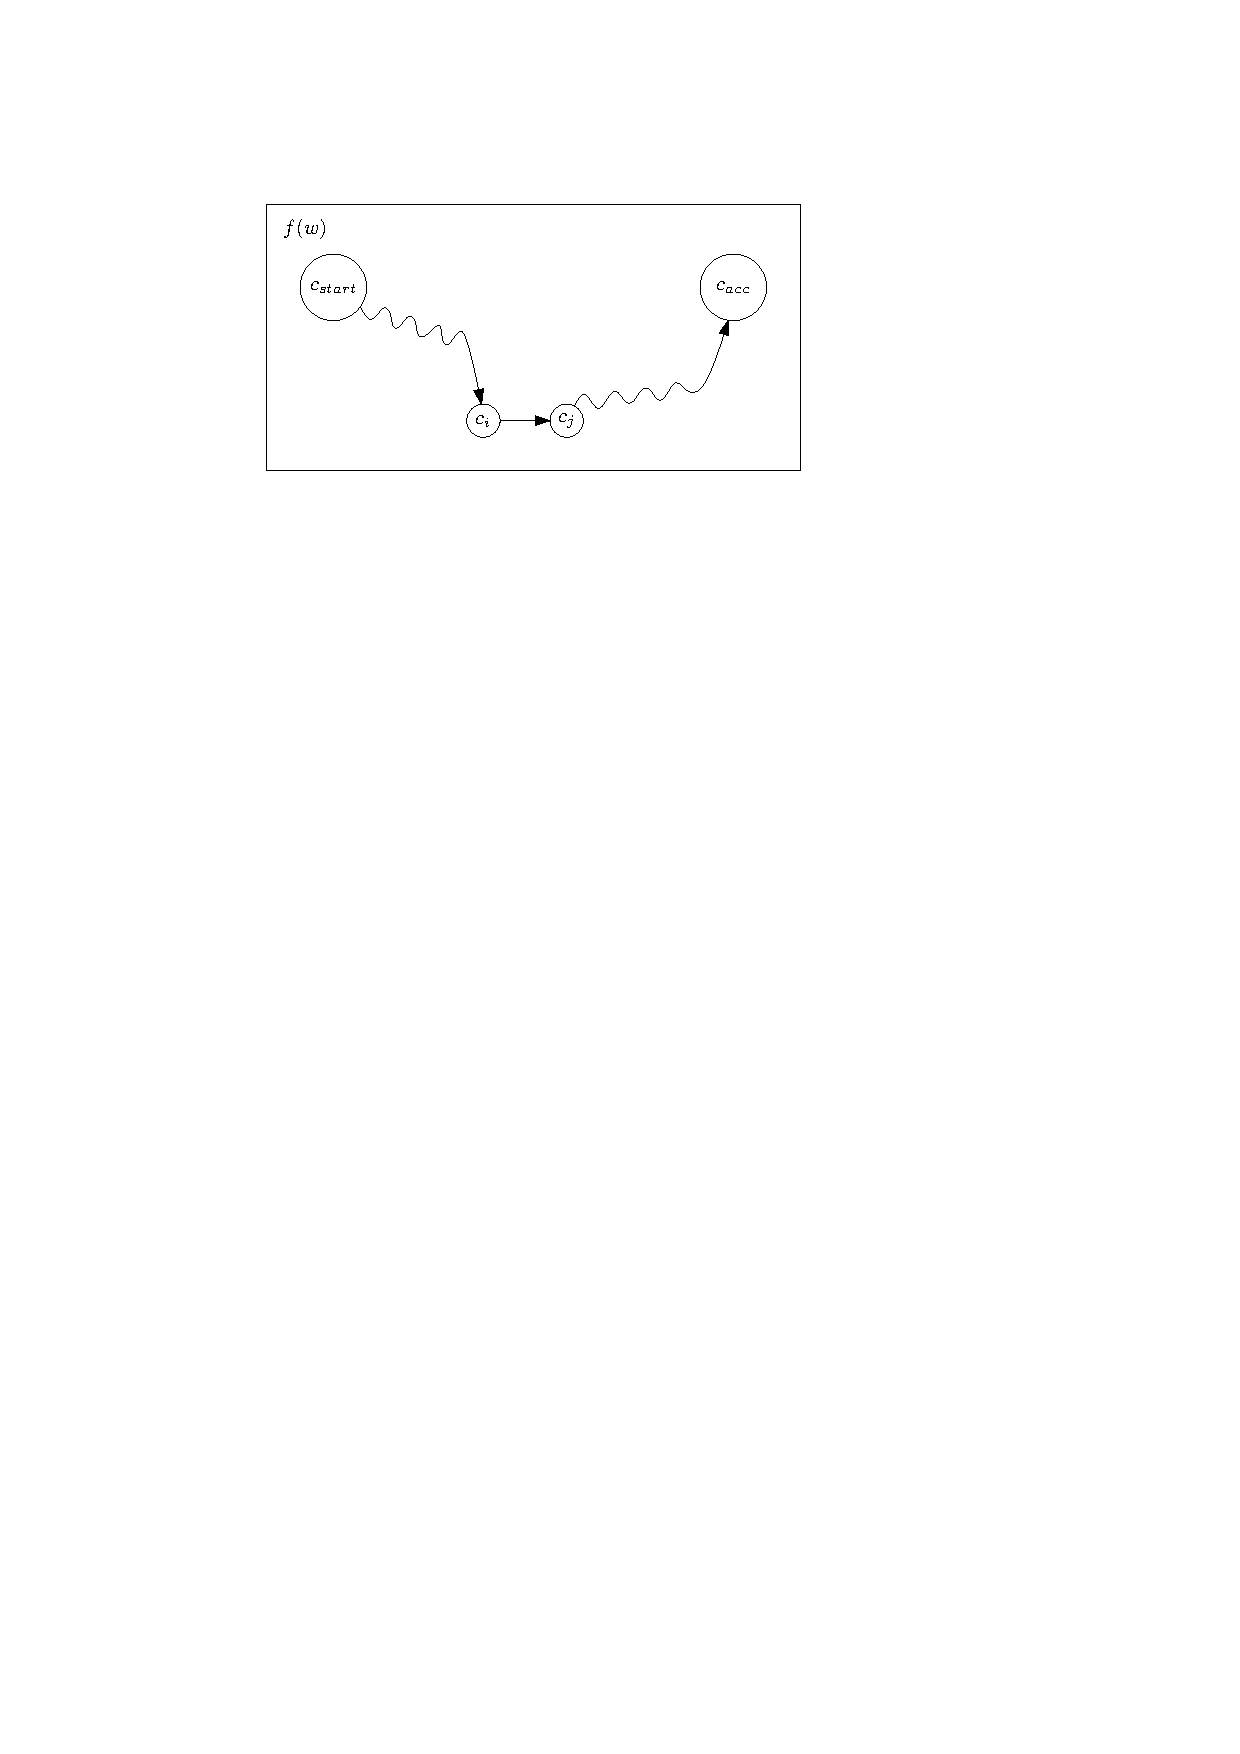
\includegraphics[width=0.4\linewidth,align=c]{computation-graph.pdf}}
        \caption{A log-space transducer for reducing $A$ to PATH and the computation graph constructed by the logspace transducer.}
        \label{fig:logspace-transducer-path}
    \end{figure}
\end{proof}

\begin{corollary}
    $
    \NLSpace \subseteq \p
    $
\end{corollary}

\begin{proof}
    A Turing machine that uses space $f(n)$ runs in time $n 2^{O(f(n))}$, so a reducer that runs in log-space also runs in polynomial time. Therefore, any language in $\NLSpace$ is polynomial time reducible to PATH, which is in $\p$.
\end{proof}

\section{NL and coNL}

\vspace{\parskip}

\begin{theorem}[Immerman-Szelepcs\'enyi (1987)]
    $\NLSpace = \coNL$
\end{theorem}